%====================== Kapitola: Číslicové signály - posloupnosti ===========================================
\chapter{Číslicové signály - posloupnosti}
\minitoc
\newpage
  Číslicové signály (matematicky posloupnosti čísel) \cite{Sovka} jsou v literatuře
  oz\-na\-čo\-vá\-ny symboly $x_n, x(n)$, nebo $x[nT]$, kde $n$ je celé číslo a označuje pořadí
  prvku v posloupnosti\footnote{Takto zavedené označení je nejednoznačné, neboť nerozlišuje mezi
  celou posloupností a jejím jediným prvkem. Posloupnost by měla být správně označena např.
  symbolem $\{x[n]\}$, zatímco symbol $x[n]$ by měl být vyhrazen pro její jeden prvek. Nicméně
  uvedené značení je všeobecně používáno.} Poslední uvedený symbol $x[nT]$ zdůrazňuje souvislost
  číslicového signálu se signálem spojitým v čase(analogovým signálem), ze kterého vznikl
  vzorkováním a kvantováním. Symbol $T$ označuje použitý \emph{vzorkovací krok}. Jeho převrácená
  hodnota je rovna \emph{vzorkovací frekvenci} $f_s=\frac{1}{T}$.

  \section{Základní typy posloupností}
    \begin{itemize}
      \item \textbf{Jednotkový impuls}
        \begin{equation}\label{SAS:eq_jednotkovy_imp}
          \delta[n]=
          \begin{cases} 
             1, &  n = 0, \\
             0, &  n \neq 0,
          \end{cases}
        \end{equation}
      \item \textbf{Jednotkový skok}
        \begin{equation}\label{SAS:eq_jednotkovy_skok}
          u[n]=
          \begin{cases} 
             1, &  n \geq 0, \\
             0, &  n < 0,
          \end{cases}
        \end{equation}
      \item \textbf{Reálná exponenciální posloupnost}
        \begin{equation}\label{SAS:eq_exp}
          x[n] = A\alpha^n, n\geq0,
        \end{equation}
      \item \textbf{Chirp signál}
        \begin{equation}\label{SAS:eq_chirp}
          x[n] = sin\left(\frac{\pi f_{max}n^2}{(N-1)f_s}\right),
        \end{equation}
        kde $f_{max}$ je maximální požadovaný kmitočet, který musí být menší než polovina
        vzorkovacího kmitočtu $f_{max}<\frac{f_s}{2}$ a $N$ je celkový počet vzorků.
      \item \textbf{Pseudonáhodná posloupnost} je posloupnost, která nahrazuje ideální bílý šum.
      Tuto posloupnost lze generovat různými algoritmy, které zaručují velmi dlouhou periodicitu
      generované posloupnosti. Má-li tato posloupnost aproximovat bílý šum, musí co nejlépe
      splňovat požadavek nekorelovanosti sousedních vzorků (tedy konstantní spektrální výkonové
      hustoty) a nulové střední hodnoty. Často je požadován i jednotkový rozptyl.
         \begin{figure}[ht!]
           \centering
           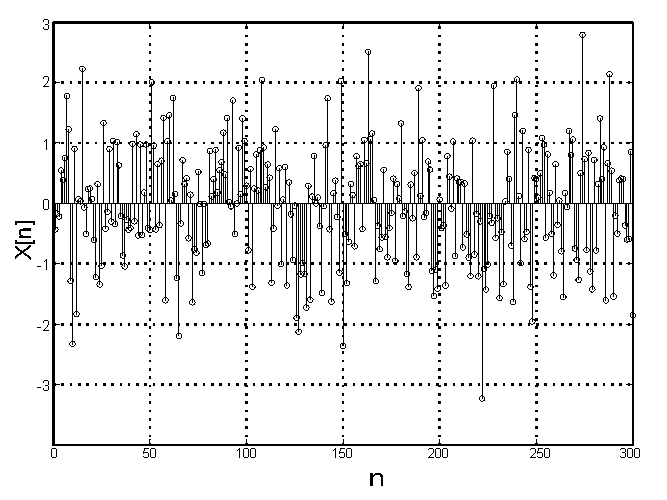
\includegraphics[width=0.8\linewidth]{randn_posloupnost.pdf}
           \caption[Příklad pseudonáhodné posloupnosti]{Příklad pseudonáhodné posloupnosti
                    generované pomocí funkce \texttt{randn(1, 300)} v MATLABu}
           \label{SAS:fig_randn}
         \end{figure}
    \end{itemize}

  \section{Generování jednoduchých signálů a jejich zobrazení v MATLABu}
    \begin{example}
      Generujte signál s lineárně rostoucím kmitočtem "\texttt{chirp signál}", maximální kmitočet
      $f_{max} = 20 Hz$, amplituda $A = 1$, vzorkovaný kmitočtem $f_s = 64 Hz$.
      \begin{figure}[!ht]
         \centering
         \begin{tabular}{c}
           \subfloat[ ]{\label{SAS:fig_chirp_stem}
             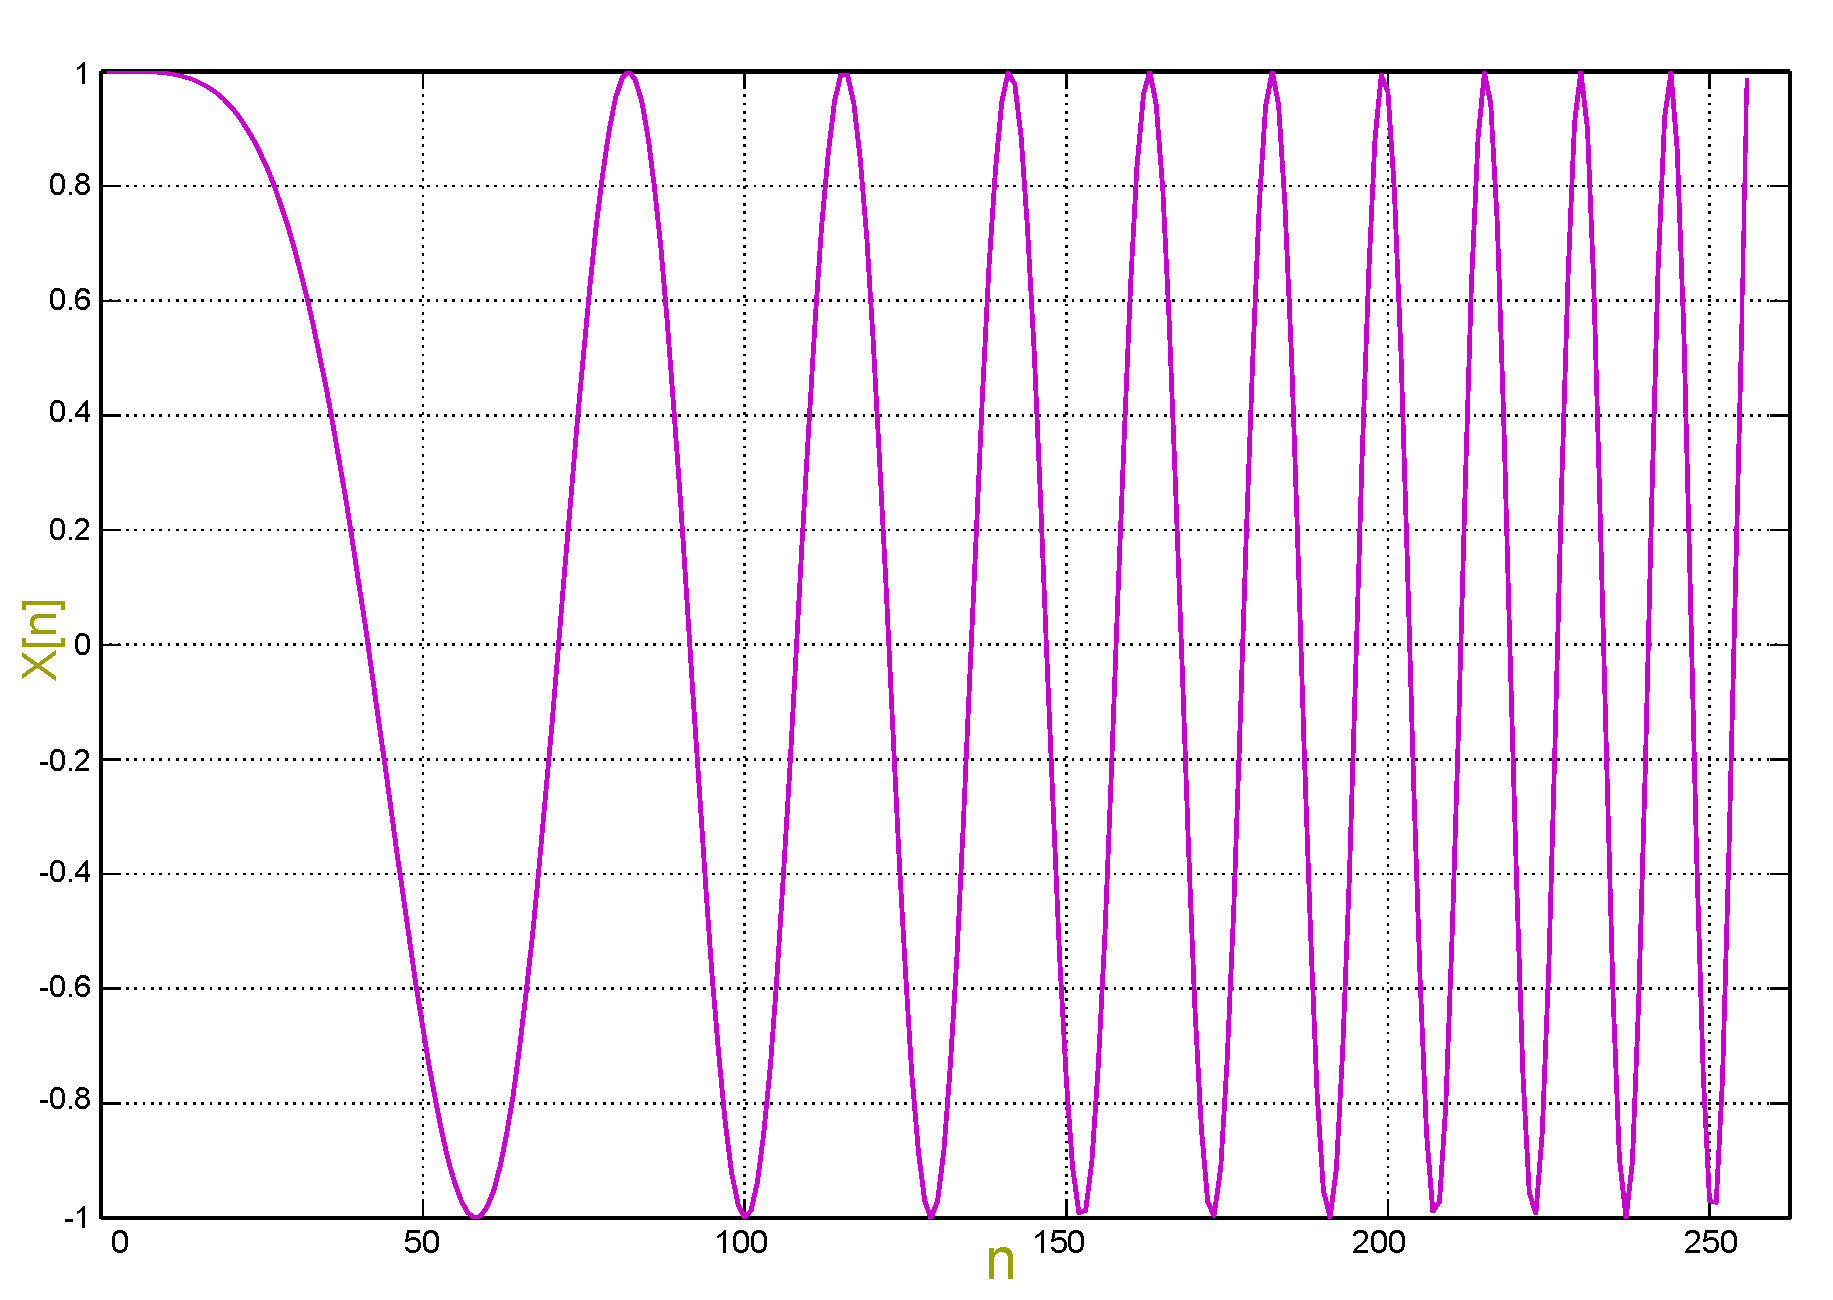
\includegraphics[width=1\linewidth]{Chirp_signal_plot.pdf}}  \\
           \subfloat[ ]{\label{SAS:fig_chirp_plot} 
             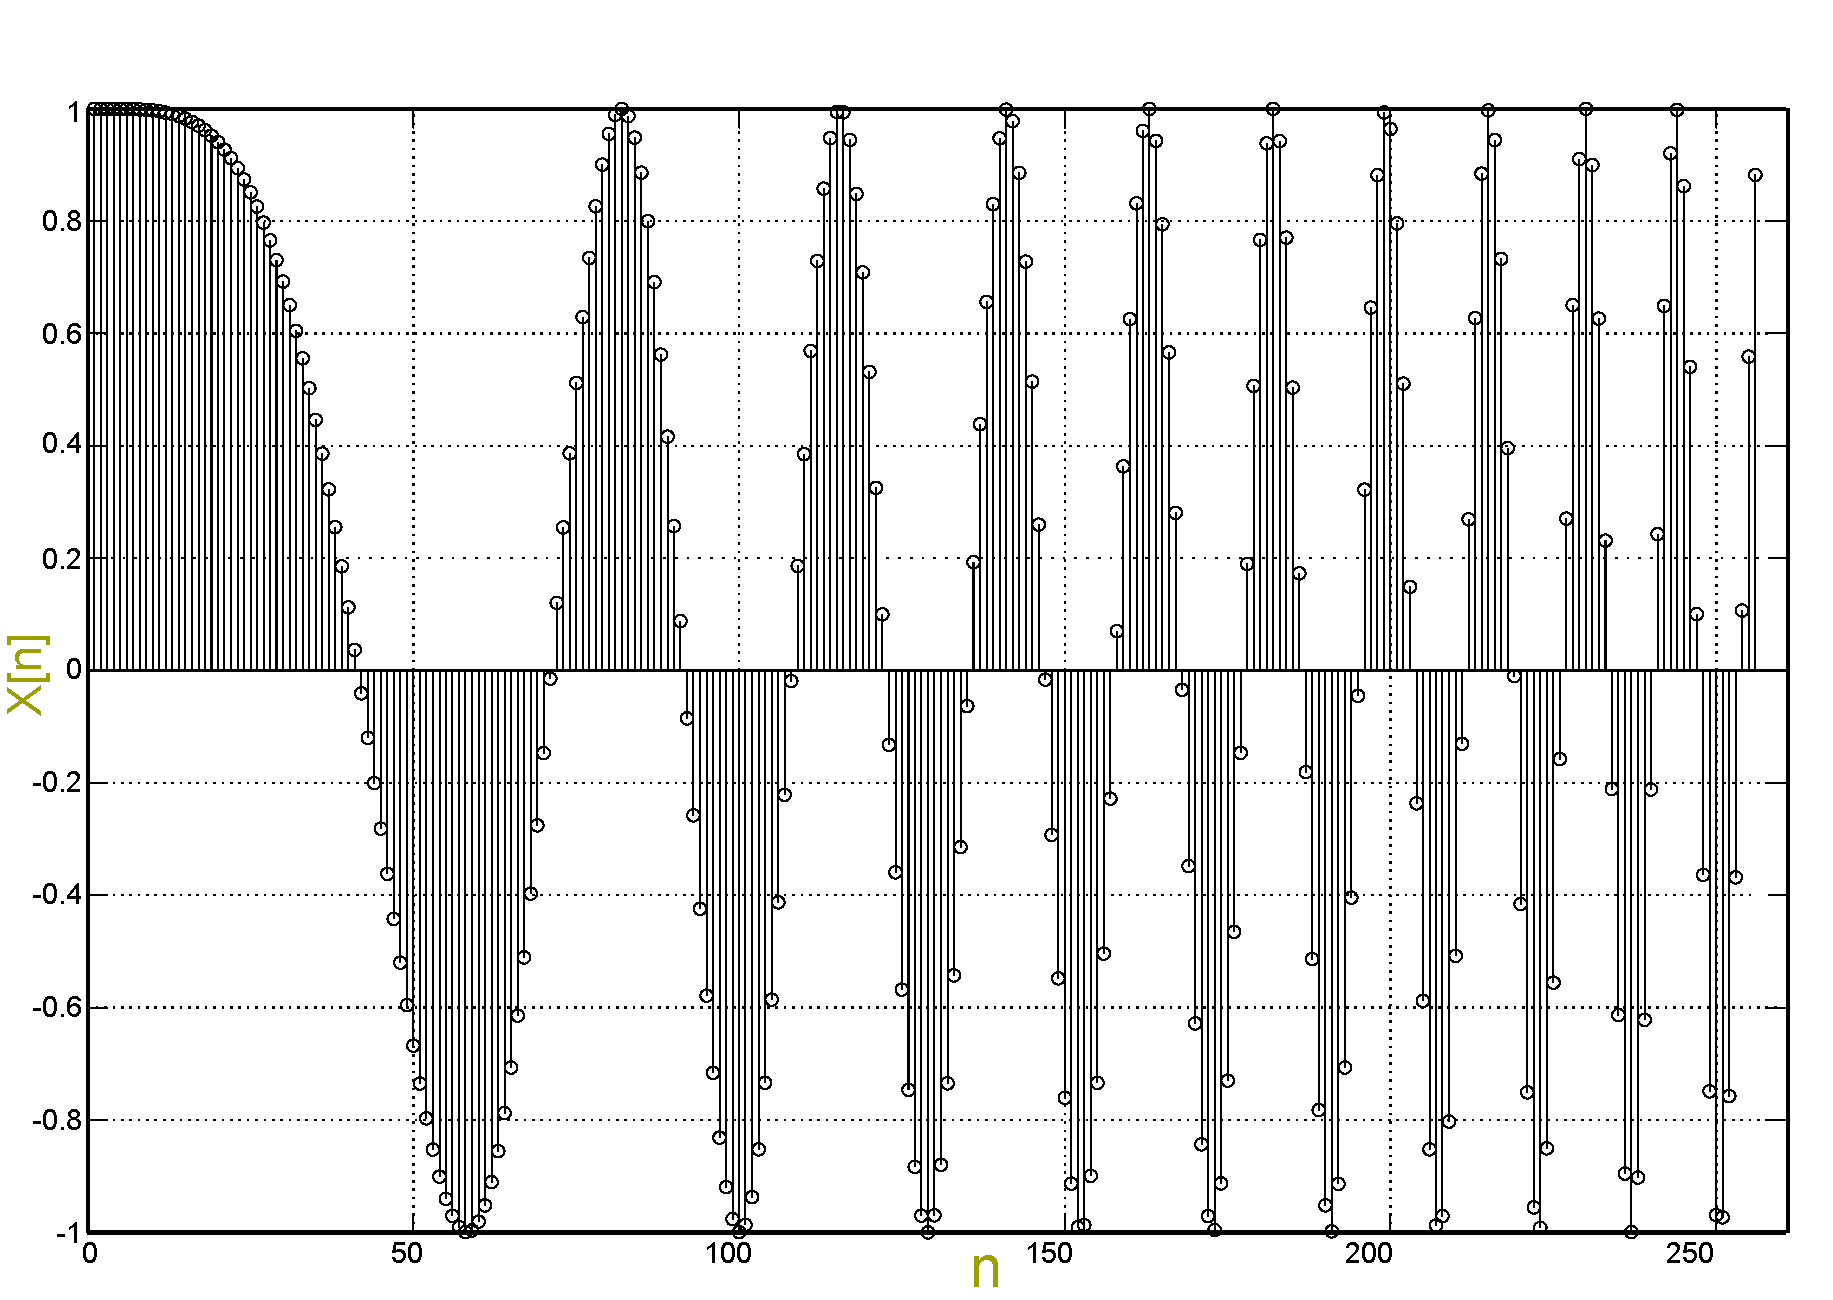
\includegraphics[width=1\linewidth]{Chirp_signal_stem.pdf}} 
         \end{tabular}  
         \caption[Chirp signál]{Chirp signál: Signál s lineárně rostoucím kmitočtem s maximální
                  frekvencí 20 Hz vzorkovaný 254 Hz. Grafická reprezentace číslicových signálů bývá
                  buď ve spojité formě (a) nebo v diskrétní formě (b) }
         \label{SAS:fig_chirp_sig}
      \end{figure}
      %---------------------------------------------------------------
      \lstinputlisting{../src/SAS/file/gen_chirp_signal.m}
      \begin{lstlisting}[caption=\texttt{gen\_chirp\_signal.m}. Generuje chirp signál]
      \end{lstlisting}
      %---------------------------------------------------------------
    \end{example}

  \section{Základní operace s posloupnosti}
    V dalším textu budeme používat tři základní lineární operace \cite{Sovka} zobrazené na
    \ref{sas:fig_zakladni_operace}:
    \begin{itemize}
      \item \texttt{součin} signálu $x[n]$ a reálné konstanty $b$:      
            $$w[n]=bx[n], n = 0,1,2, \ldots$$ Tato operace je v praxi realizována násobičkou a je
            zdrojem numerických chyb, tedy kvantizačního šumu, který produkují číslicová zařízení.
      \item \texttt{součet} signálu $x[n]$ a signálu $y[n]$:           
            $$v[n]=x[n]+y[n], n = 0,1,2, \ldots$$ Tuto operaci provádí sčítačka. Při neošetření může
            tato operace generovat hrubé chyby.
      \item \texttt{zpoždění} signálu $x[n]$ o $k$ vzorkovacích kroků:  
            $$y[n]=x[n-k], n = 0,1,2, \ldots, n = 1,2, \ldots, M $$  Hodnoty $x[-k], k = 1, 2,
            \ldots, M$ se nazývají \emph{počáteční podmínky}. V digitálních implementací provádíme
            operaci zpoždění paměťového registru pro každou jednotku požadovaného zpoždění $z^{-1}$.
    \end{itemize}

    \begin{figure}[ht!]
      \centering
      \begin{tabular}{c}
        \hspace{0.1cm}
        \subfloat[ ]   {
          \begin{tikzpicture}[scale=1,>=latex']
  \coordinate (A) at (-1,-1.5) {};
  \coordinate (B) at (-1,-2.5) {};
  \coordinate (C) at (0,-2) {};    
  \coordinate (D) at ($ (A)!0.5!(B) $) {};
    \fill[fill=blue!20!white, draw=blue!50!black, very thick] (A) -- (B) -- (C) -- (A);
    \node[] at ($ (D)!0.4!(C) $) {\(b\)};
    \draw[->] (C) ++ (-2,0)  node[left] {\(x[n]\)} -- (D);
    \draw[->] (C) -+ (1,-2) node[right] {\(bx[n]\)}; 
\end{tikzpicture}}  \\
        \subfloat[ ]   {
          \begin{tikzpicture}[scale=1,>=latex']
  \coordinate (A) at (0,0) {};
  \coordinate (B) at (1,-1) {};   
  \coordinate (C) at ($ (A)!0.5!(B) $) {};   
  \coordinate (D) at (A |- C) {}; 
    \fill[fill=blue!20!white, draw=blue!50!black, very thick] (A) circle (0.5);
    \node[] at (A) {\(+\)};
    \draw[->] (-1.5,0) node[left] {\(x[n]\)} -- (-0.5,0);
    \draw[->] (0,1.5) node[above] {\(y[n]\)} -- (0,0.5);
    \draw[->] (0.5,0) --+ (1,0) node[right] {\(x[n]+y[n]\)}; 
\end{tikzpicture}
}  \\
        \subfloat[ ]   {
          \begin{tikzpicture}[scale=1,>=latex']
  \coordinate (A) at (0,0) {};
  \coordinate (B) at (1,-1) {};   
  \coordinate (C) at ($ (A)!0.5!(B) $) {};   
  \coordinate (D) at (A |- C) {}; 
    \fill[fill=blue!20!white, draw=blue!50!black, very thick] (A) rectangle (B);
    \node[] at (C) {\(z^{-k}\)};
    \draw[->] (D) + (-1,0) node[left] {\(x[n]\)} -- (D);
    \draw[->] (D) ++(1,0) --+ (1,0) node[right] {\(x[n-k]\)}; 
\end{tikzpicture}}    
      \end{tabular}
      \caption[Základní operace]{Symboly základních operací} 
      \label{sas:fig_zakladni_operace} 
    \end{figure}    